\begin{theappendices}

\chapter{Model Training Details}

\section{Hardware Specifications}
The experiments in this study were conducted using the following hardware configuration:
\begin{itemize}
    \item GPU: NVIDIA Tesla V100 with 32GB memory
    \item CPU: Intel Xeon Silver 4210
    \item RAM: 16GB
    \item Storage: 500GB SSD for data caching
\end{itemize}

\section{Training Hyperparameters}
The models were trained using the following hyperparameters:
\begin{table}[h]
    \centering
    \caption{Training Hyperparameters for AS-Net Variants}
    \label{tab:training_hyperparams}
    \begin{tabular}{|l|c|}
        \hline
        \textbf{Parameter} & \textbf{Value} \\
        \hline
        Optimizer & Adam \\
        Learning Rate & 1e-4 (initial) \\
        Batch Size (per replica) & 32 (VGG16), 4 (Lightweight Models) \\
        Maximum Epochs & 30 \\
        Early Stopping Patience & 15 epochs (monitoring \texttt{val\_loss}) \\
        Learning Rate Reduction & ReduceLROnPlateau (factor=0.5, patience=5 on \texttt{val\_loss}) \\
        Loss Function & Combined Loss: 0.5*WBCE + 0.5*Dice Loss \\
        WBCE Class Weight & 100 for tumor class \\
        Best Checkpoint Monitor & \texttt{val\_dice\_coef} (mode='max') \\
        \hline
    \end{tabular}
\end{table}

\section{Data Preprocessing}
The preprocessing of BraTS 2023-GLI (Task 1) NIfTI files into H5 slices involved:
\begin{itemize}
    \item Extraction of 2D axial slices from 3D volumes
    \item Z-score normalization of MRI modalities (T1ce, FLAIR) per slice, per modality
    \item Mapping of selected MRI modalities to RGB channels: [T1ce, FLAIR, T1ce]
    \item Conversion of multi-class tumor labels (NCR/NET, ED, ET) into a single binary segmentation mask (Tumor vs. Background)
    \item Resizing input images and masks to target dimensions specific to each encoder (VGG16, MNv3-L/S, ENv2-B0: 224x224; ENv2-B1: 240x240) using appropriate interpolation (Bilinear for image, Nearest Neighbor for mask).
\end{itemize}

\chapter{Implementation Code Snippets}

\section{Combined Loss Function Implementation}
The custom loss function combined weighted binary cross-entropy with the Dice loss to address class imbalance:

\begin{verbatim}
def weighted_bce_dice_loss(y_true, y_pred, weight=100.0):
    # Weighted binary cross entropy component
    bce = tf.keras.losses.binary_crossentropy(y_true, y_pred)
    weight_mask = tf.where(y_true > 0.5, weight, 1.0)
    weighted_bce = bce * weight_mask
    weighted_bce_loss = tf.reduce_mean(weighted_bce)
    
    # Dice loss component
    dice_loss = 1 - dice_coef(y_true, y_pred)
    
    # Combined loss
    combined_loss = 0.5 * weighted_bce_loss + 0.5 * dice_loss
    return combined_loss
\end{verbatim}

\section{Evaluation Metrics Implementation}
The key metrics used for model evaluation were implemented as follows:

\begin{verbatim}
def dice_coef(y_true, y_pred, smooth=1.0):
    y_true_f = tf.reshape(y_true, [-1])
    y_pred_f = tf.reshape(y_pred, [-1])
    intersection = tf.reduce_sum(y_true_f * y_pred_f)
    return (2. * intersection + smooth) / (
        tf.reduce_sum(y_true_f) + tf.reduce_sum(y_pred_f) + smooth)

def iou_coef(y_true, y_pred, smooth=1.0):
    y_true_f = tf.reshape(y_true, [-1])
    y_pred_f = tf.reshape(y_pred, [-1])
    intersection = tf.reduce_sum(y_true_f * y_pred_f)
    union = tf.reduce_sum(y_true_f) + tf.reduce_sum(y_pred_f) - intersection
    return (intersection + smooth) / (union + smooth)
\end{verbatim}

\chapter{AS-Net Module Configurations}

\section{Spatial Attention Module (SAM) Configuration}
The SAM module used the following key configurations:
\begin{itemize}
    \item Feature refinement path with three 3×3 convolutions (F'(X))
    \item Feature extraction path with one 1×1 convolution (F''(X))
    \item Multi-scale spatial attention with max-pooling at scales 2×2 and 4×4
    \item Element-wise multiplication of refined features with spatial attention map
    \item Residual connection from feature extraction path
\end{itemize}

\section{Channel Attention Module (CAM) Configuration}
The CAM module used the following configurations:
\begin{itemize}
    \item Feature refinement path with three 3×3 convolutions (F'(X))
    \item Feature extraction path with one 1×1 convolution (F''(X))
    \item Global average pooling for channel statistics
    \item Two-layer MLP with reduction ratio = 16 for generating channel weights
    \item Element-wise multiplication for channel recalibration
    \item Residual connection from feature extraction path
\end{itemize}

\section{Synergy Module Configuration}
The Synergy module used the following configuration:
\begin{itemize}
    \item Learnable scalar weights (α, β) for balancing SAM and CAM features
    \item Adaptive fusion of spatial and channel attention features
    \item 1×1 convolution for feature refinement after fusion
    \item Batch normalization for stabilizing training
\end{itemize}

\chapter{Encoder Integration Details}

\section{Skip Connection Layers}
The specific encoder layers used for skip connections with the AS-Net decoder:

\begin{table}[h]
    \centering
    \caption{Encoder Skip Connection Layer Names}
    \label{tab:skip_connections}
    \resizebox{\textwidth}{!}{%
    \begin{tabular}{|l|c|c|c|c|}
        \hline
        \textbf{Encoder} & \textbf{Skip 1} & \textbf{Skip 2} & \textbf{Skip 3} & \textbf{Skip 4} \\
        \hline
        VGG16 & \texttt{block1\_conv2} & \texttt{block2\_conv2} & \texttt{block3\_conv3} & \texttt{block4\_conv3} \\
        MobileNetV3-Large & \texttt{re\_lu\_2} & \texttt{re\_lu\_5} & \texttt{re\_lu\_11} & \texttt{re\_lu\_14} \\
        MobileNetV3-Small & \texttt{re\_lu\_1} & \texttt{re\_lu\_3} & \texttt{re\_lu\_8} & \texttt{re\_lu\_10} \\
        EfficientNetV2-B0 & \texttt{block1a\_project\_bn} & \texttt{block2b\_add} & \texttt{block4a\_project\_bn} & \texttt{block6a\_project\_bn} \\
        EfficientNetV2-B1 & \texttt{block1b\_add} & \texttt{block2c\_add} & \texttt{block4c\_add} & \texttt{block6d\_add} \\
        \hline
    \end{tabular}%
    }
    \footnotesize{\\ Note: Layer names are indicative and depend on the specific Keras implementation. Verification against model summaries is recommended.}
\end{table}

\section{Fine-Tuning Strategies}
The fine-tuning approach used for each encoder backbone:

\begin{table}[h]
    \centering
    \caption{Encoder Fine-Tuning Strategies}
    \label{tab:fine_tuning}
    \resizebox{\textwidth}{!}{%
    \begin{tabular}{|l|c|c|}
        \hline
        \textbf{Encoder} & \textbf{Frozen Layers (Approx.)} & \textbf{Trainable Layers (Approx.)} \\
        \hline
        VGG16 & Up to \texttt{block3\_conv3} & From \texttt{block4\_conv1} onwards \\
        MobileNetV3-Large & Up to block \texttt{expanded\_conv\_5} & From block \texttt{expanded\_conv\_6} onwards \\
        MobileNetV3-Small & Up to block \texttt{expanded\_conv\_3} & From block \texttt{expanded\_conv\_4} onwards \\
        EfficientNetV2-B0 & Up to block \texttt{block3b} & From block \texttt{block4a} onwards \\
        EfficientNetV2-B1 & Up to block \texttt{block3c} & From block \texttt{block4a} onwards \\
        \hline
    \end{tabular}%
    }
     \footnotesize{\\ Note: Specific layer names/indices defining the boundary between frozen and trainable layers may vary slightly based on implementation details.}
\end{table}

\chapter{Detailed Test Results}
\label{app:detailed_results}

This section provides the detailed performance metrics for each model variant evaluated on the test set, corresponding to the best checkpoint saved during training based on \texttt{val\_dice\_coef} (validation Dice coefficient).

\begin{table}[h]
    \centering
    \caption{Detailed Test Metrics per Model Variant}
    \label{tab:detailed_validation_metrics} % Note: Label kept same for consistency if referenced elsewhere, but caption changed.
    \resizebox{\textwidth}{!}{%
    \begin{tabular}{|l|c|c|c|c|c|c|}
        \hline
        \textbf{Encoder Backbone} & \textbf{Input Size} & \textbf{Dice Coef / F1} & \textbf{IoU} & \textbf{Precision} & \textbf{Recall} & \textbf{Binary Acc.} \\
        \hline
        VGG16 & 224x224 & 0.8873 & 0.7974 & 0.8334 & 0.9487 & 0.9974 \\
        MobileNetV3-Large & 224x224 & 0.8738 & 0.7759 & 0.8186 & 0.9371 & 0.9971 \\
        MobileNetV3-Small & 224x224 & 0.8570 & 0.7498 & 0.7912 & 0.9348 & 0.9967 \\
        EfficientNetV2-B0 & 224x224 & 0.8853 & 0.7942 & 0.8327 & 0.9451 & 0.9974 \\
        EfficientNetV2-B1 & 240x240 & 0.8815 & 0.7881 & 0.8185 & 0.9550 & 0.9973 \\
        \hline
    \end{tabular}%
    }
    \footnotesize{\\ Note: Metrics obtained from evaluating the best checkpoint (selected based on validation performance) on the test split of the BraTS 2023-GLI (Task 1) dataset.}
\end{table}

\chapter{Supplementary Figures}
\label{app:supplementary_figures}

\section{Training History Plots}
This section contains the training history plots for all evaluated model variants, showing key metrics over epochs. Figure \ref{fig:training_plots_placeholder} in Chapter 4 shows examples for VGG16 and EfficientNetV2-B0.

\begin{figure}[ht]
    \centering
    \IfFileExists{figures/training-history-plots/placeholder_training_plot_mnv3l.png}{%
        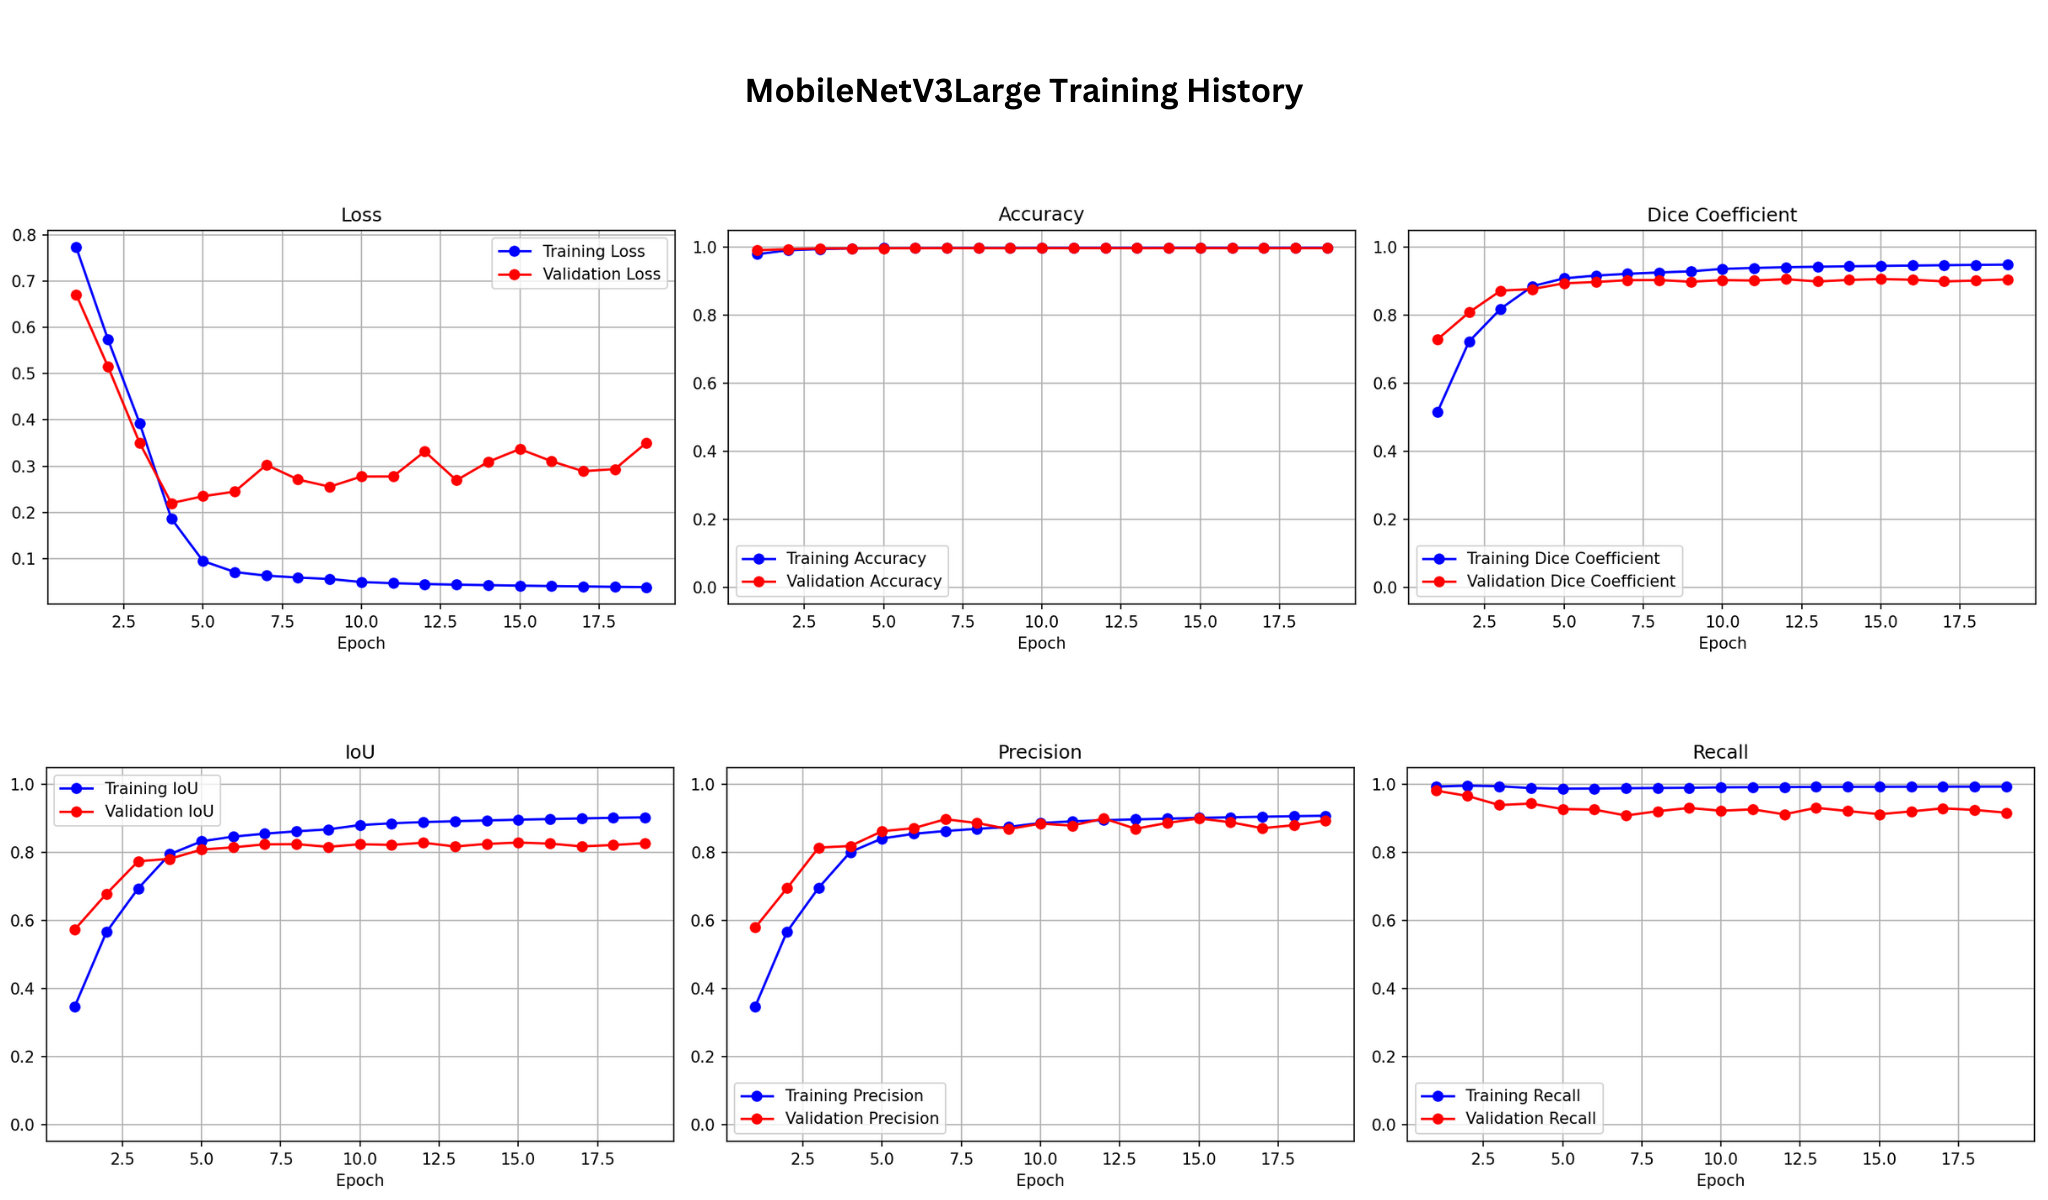
\includegraphics[width=0.9\textwidth]{figures/training-history-plots/placeholder_training_plot_mnv3l.png}
    }{%
        \fbox{\begin{minipage}{0.9\textwidth}\centering[MobileNetV3-Large Training Plot Placeholder]\end{minipage}}
    }
    \caption{Training history plot for AS-Net with MobileNetV3-Large encoder.}
    \label{fig:training_plot_mnv3l}
\end{figure}

\begin{figure}[ht]
    \centering
    \IfFileExists{figures/training-history-plots/placeholder_training_plot_mnv3s.png}{%
        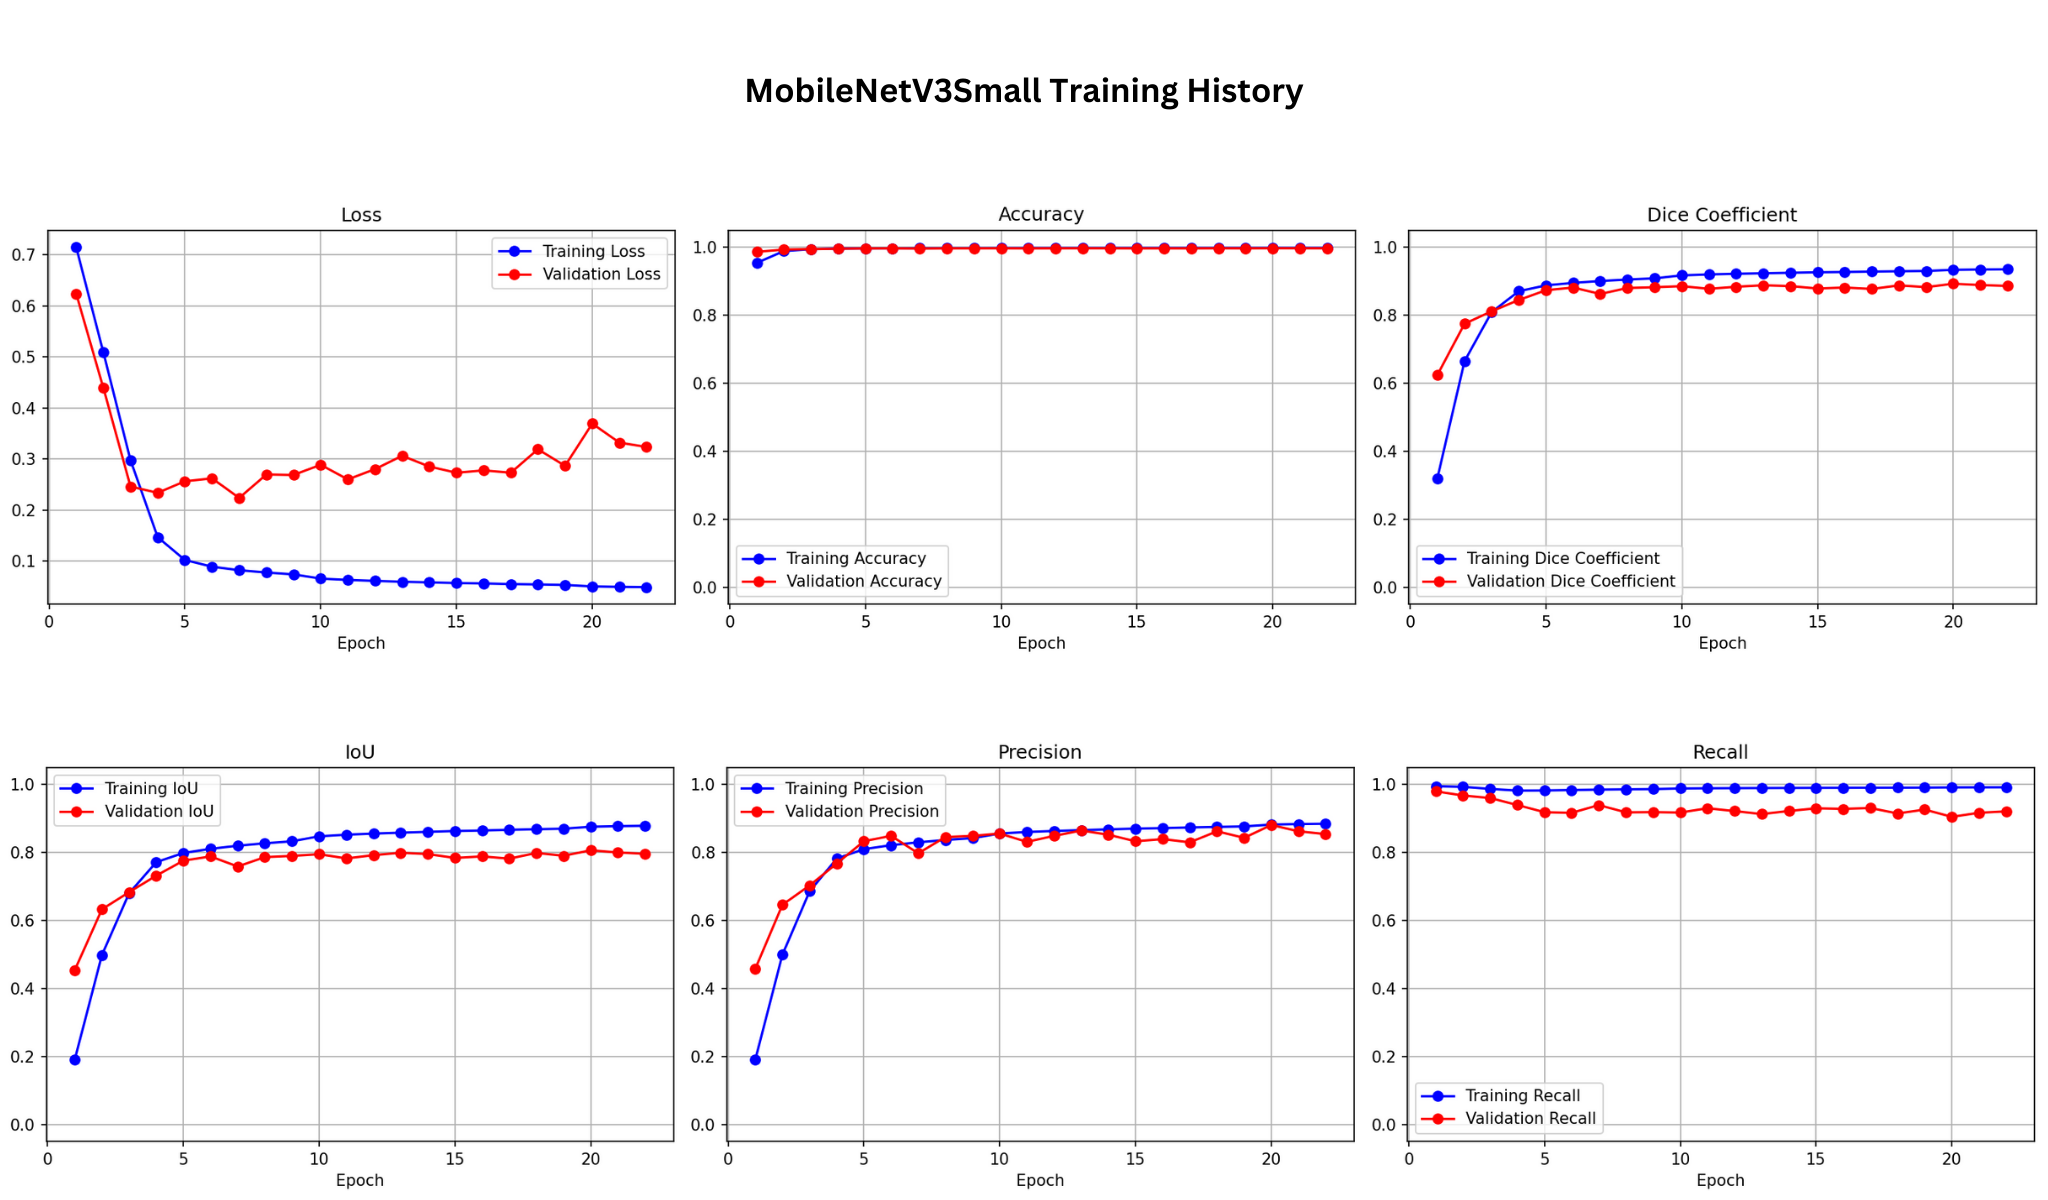
\includegraphics[width=0.9\textwidth]{figures/training-history-plots/placeholder_training_plot_mnv3s.png}
    }{%
        \fbox{\begin{minipage}{0.9\textwidth}\centering[MobileNetV3-Small Training Plot Placeholder]\end{minipage}}
    }
    \caption{Training history plot for AS-Net with MobileNetV3-Small encoder.}
    \label{fig:training_plot_mnv3s}
\end{figure}

\begin{figure}[ht]
    \centering
    \IfFileExists{figures/training-history-plots/placeholder_training_plot_env2b1.png}{%
        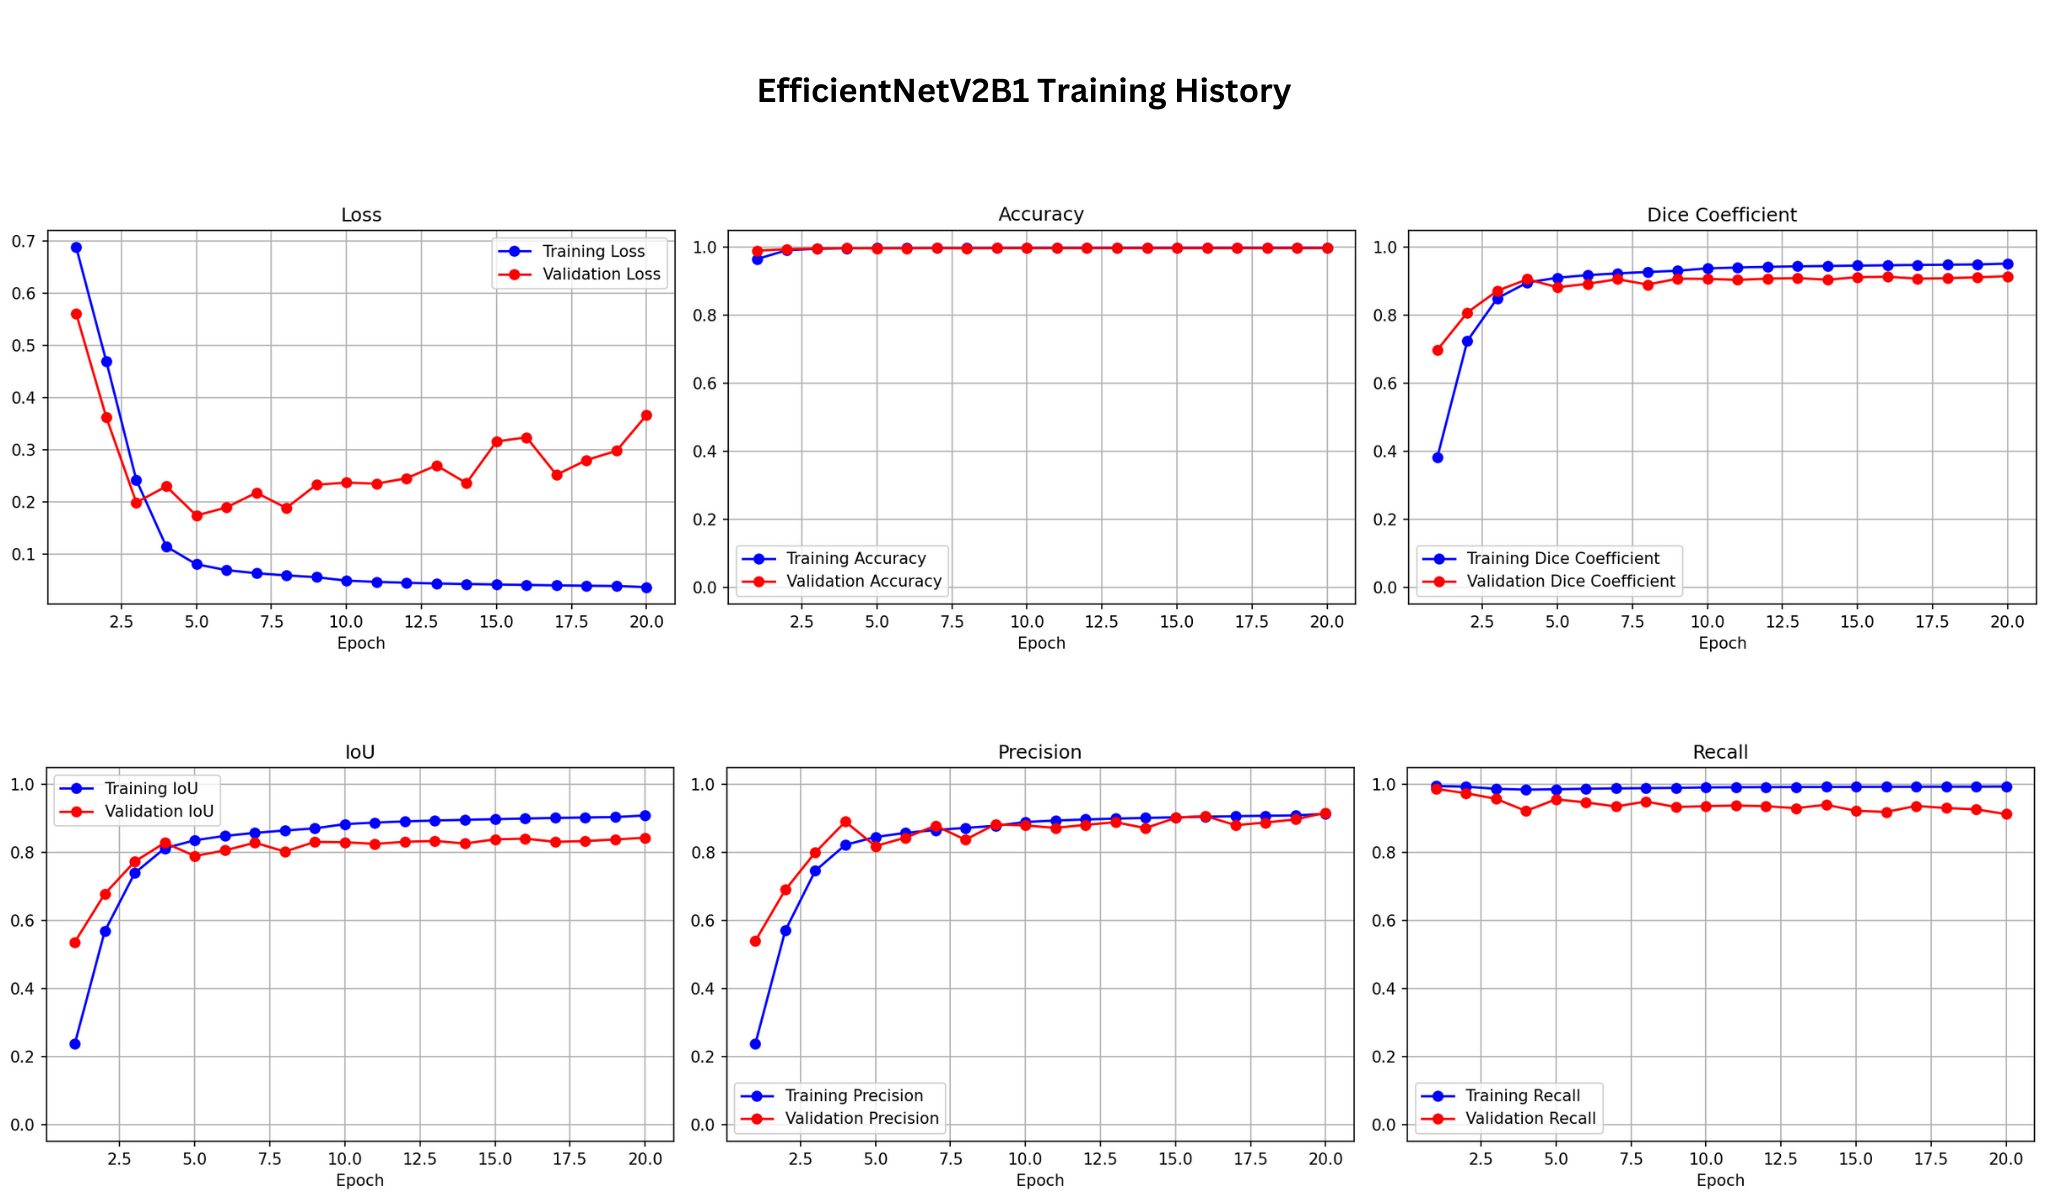
\includegraphics[width=0.9\textwidth]{figures/training-history-plots/placeholder_training_plot_env2b1.png}
    }{%
        \fbox{\begin{minipage}{0.9\textwidth}\centering[EfficientNetV2-B1 Training Plot Placeholder]\end{minipage}}
    }
    \caption{Training history plot for AS-Net with EfficientNetV2-B1 encoder.}
    \label{fig:training_plot_env2b1}
\end{figure}

% \section{Qualitative Segmentation Examples}
% This section provides additional visual examples of segmentation results from the validation set for different model variants.

% \begin{figure}[ht]
%     \centering
%     \IfFileExists{figures/placeholder_segmentation_examples.png}{%
%         \includegraphics[width=0.9\textwidth]{figures/placeholder_segmentation_examples.png}
%     }{%
%         \fbox{\begin{minipage}{0.9\textwidth}\centering[Segmentation Examples Placeholder: Input MRI, Ground Truth, VGG16 Pred, ENv2-B0 Pred, etc.]\end{minipage}}
%     }
%     \caption{Example segmentation results on validation slices comparing different AS-Net variants.}
%     \label{fig:segmentation_examples_appendix}
% \end{figure}

\end{theappendices}